\documentclass[12pt,a4paper]{report}
\usepackage[utf8]{inputenc}
\usepackage{amsmath}
\usepackage{algorithm}
\usepackage{algpseudocode}
\usepackage{amssymb}
\usepackage{graphicx}
\usepackage{geometry}
\usepackage[hidelinks]{hyperref}  % For clickable references
\usepackage[capitalise]{cleveref}  % For intelligent cross-referencing
\usepackage[english]{babel}

\usepackage{makecell}
\usepackage{caption}
\usepackage{array}
\usepackage{listings}
\usepackage{titlesec}
\usepackage{hyperref}
\hypersetup{
	colorlinks=true,
	linkcolor=black,
	filecolor=black,      
	urlcolor=cyan,
	citecolor=black
}

\graphicspath{{C:/Users/frabb/OneDrive - Cal Poly/Documents (Cloud)/0 CALPOLY/000Thesis/Chapters/Images/}}

\geometry{
	top=1in,
	bottom=1in,
	left=1.5in,
	right=1in
}

% Remove space before equations only
\makeatletter
\g@addto@macro\normalsize{%
	\setlength\abovedisplayskip{-10pt}
	\setlength\abovedisplayshortskip{-10pt}
}
\makeatother

% Updated list settings
\usepackage{enumitem}
\setlist[itemize]{nosep, leftmargin=*}
\setlist[enumerate]{nosep, leftmargin=*}

% Remove space before lists
\usepackage{etoolbox}
\BeforeBeginEnvironment{itemize}{\vspace{-\baselineskip}}
\BeforeBeginEnvironment{enumerate}{\vspace{-\baselineskip}}

\setlength{\parskip}{\baselineskip}
\titlespacing*{\section}{0pt}{0pt}{0pt}
\titlespacing*{\section}{0pt}{0pt}{-10pt}
\titlespacing*{\subsection}{0pt}{0pt}{-10pt}

\captionsetup[table]{skip=0pt}

\usepackage{xcolor}

\definecolor{codegreen}{rgb}{0,0.6,0}
\definecolor{codegray}{rgb}{0.5,0.5,0.5}
\definecolor{codepurple}{rgb}{0.58,0,0.82}
\definecolor{backcolour}{rgb}{0.95,0.95,0.92}

\lstdefinestyle{mystyle}{
	backgroundcolor=\color{backcolour},   
	commentstyle=\color{codegreen},
	keywordstyle=\color{magenta},
	numberstyle=\tiny\color{codegray},
	stringstyle=\color{codepurple},
	basicstyle=\ttfamily\footnotesize,
	breakatwhitespace=false,         
	breaklines=true,                 
	captionpos=b,                    
	keepspaces=true,                 
	numbers=left,                    
	numbersep=5pt,                  
	showspaces=false,                
	showstringspaces=false,
	showtabs=false,
	tabsize=2
}

\lstset{style=mystyle}

\title{Tutorial}
\author{Jakob Frabosilio}
\date{\today}
\setcounter{chapter}{4}
\begin{document}

\chapter{Kalman Filtering} \label{chap:5c}
The acoustic positioning system described in Chapter \ref{chap:3c} returns a single position estimate for one acoustic pulse recording. The dead reckoning system described in Chapter \ref{chap:4c} provides a single change-in-position estimate for each acoustic position estimate. In this chapter, these two measurements are combined over time with a mathematical tool known as a Kalman filter. The Kalman filter makes use of the dynamics of the iSBL system and helps combat the noise between individual position estimates, and is an indispensable tool for parameter estimation and signal filtering.

The first section of this chapter provides a theoretical overview of the Kalman filter; this is followed by the Kalman filter’s software implementation in this thesis. Next, two separate Kalman filter systems are designed: one for filtering only acoustic position estimates, and one for combining the acoustic position estimates with the dead reckoning estimates (iSBL-SF). Finally, the tuning of these two systems is briefly discussed, with recommendations for future implementations.

\section{Kalman Filter Overview} \label{sec:5s1}
The Kalman filter was primarily developed by Rudolf E. Kálmán, a Hungarian-American engineer, in 1960. Kálmán presents a solution for the filtering of linear systems, attempting to separate random noise from signals in an optimal way. The derivation of this solution will not be presented here - the original paper by Kálmán is available in the references of this thesis \cite{kalman}.

\subsection{Kalman Filter Applications} \label{ssec:5s1s1}
Kalman filters are very commonly used in controls engineering solutions; the filter has applications in a wide variety of fields, including autonomous vehicle research, guidance, navigation, and control (GNC) systems, stock market prediction, and computer vision. In general, Kalman filters are extremely useful for filtering noisy data when the dynamics of the system are known \cite{kalmanapps}. Another extremely powerful function of the Kalman filter is estimating unmeasurable states of a system; for example, estimating the speed of a vehicle using the measured GPS position over time, without measuring the speed directly. This function will not be used in this implementation, but it is perhaps the most useful component of Kalman filters in controls engineering.

The Kalman filter assumes that the dynamics of the system can be described with a set of linear equations; frequently, the state-space representation of the system is used. Modifications of the basic Kalman filter are a common area of research. The extended Kalman filter was devised to work with non-linear systems and has many variants, like the unscented Kalman filter, that improve upon it with higher computational efficiency \cite{kfsimply}. Extended Kalman filters are possibly the most common sensor fusion algorithm used for computing an orientation estimate for MEMS IMUs \cite{madgwick} (see Section \ref{ssec:4s1s2}), and are used frequently in autonomous underwater vehicle positioning \cite{tightekf} \cite{iusblukf}. 

The implementation in this thesis uses a standard Kalman filter, as the movement of the iSBL array can be described using a linear state-space model. The system dynamics of the iSBL array assume a constant-velocity model for simplicity. Of course, this assumption is not necessarily true; otherwise, the Fo-SHIP end effector would never be able to move the iSBL array to different positions! However, the acceleration of the platform can be considered as random noise; with this assumption, the acceleration does not need to be directly measured or estimated. This assumption is necessary to make the system linear and to prevent the need for an extended Kalman filter. The implementation of an extended Kalman filter is much more complex than a standard Kalman filter, and was deemed out-of-scope for this thesis. For a full underwater implementation, using a model that tracks acceleration as a state variable would be highly encouraged. This could be implemented as a tightly-coupled extended Kalman filter that combines the acoustic positioning estimate with the IMU measurements more directly, like the approach used by Morgado, Oliveira, and Silvestre \cite{tightekf}.

\subsection{Kalman Filter Functional Explanation} \label{ssec:5s1s2}
The theory of the Kalman filter is relatively complex and appears daunting for the uninitiated; thankfully, online sources like engineer William Franklin’s website provide a simple explanation of the Kalman filter \cite{kfsimply}. The functional explanation below builds primarily off of Franklin’s work.

The Kalman filter consists of three primary steps: the initialization step, the prediction step, and the update step. Figure \ref{fig:kalmanbd} provides a graphical representation of the process. In this figure, the initialization step occurs in blocks 1 and 2, the prediction step occurs in block 3, and the update step occurs in blocks 4 and 5. Note that the graphical representation uses the matrix \(\mathbf{A}\) to represent the state transition matrix, while this explanation uses the matrix \(\mathbf{F}\). Also note that the graphical representation describes the system in terms of the current iteration \(k\) and the previous iteration \(k-1\), while this explanation uses the next iteration \(k+1\) and the current iteration \(k\).

\pagebreak

\begin{figure}[htbp]
	\centering
	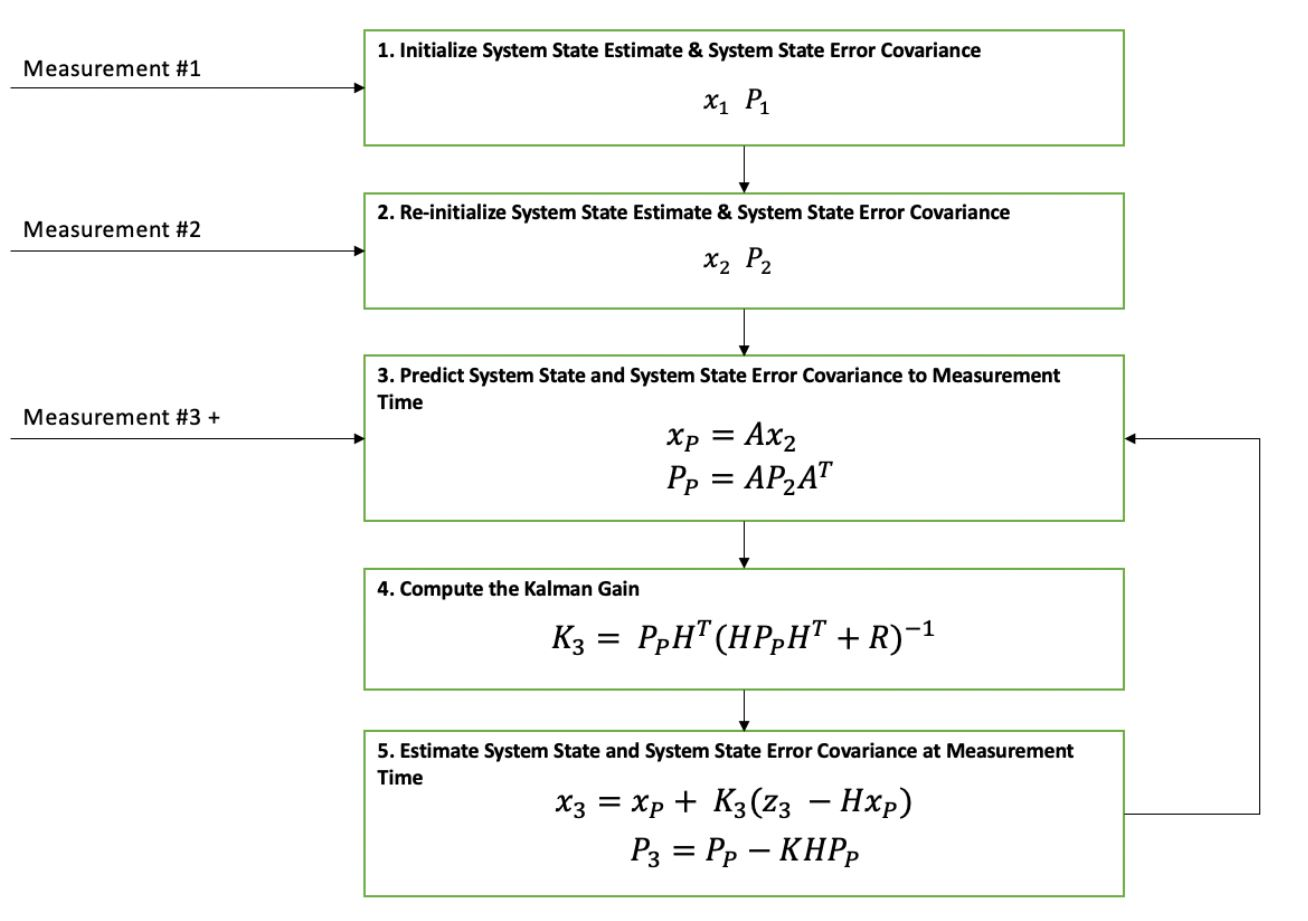
\includegraphics[width=\textwidth]{kalmanbd}
	\caption{Kalman filter block diagram \cite{kfsimply}}
	\label{fig:kalmanbd}
\end{figure}

For the remainder of this section, an example will be used to help explain how a Kalman filter works. Imagine a plane flying along a straight line. The plane has a GPS receiver that can return a position estimate along this line relative to some starting position. The plane also has a pitot tube that measures the air pressure outside the airplane; this can be converted to relative velocity using Bernoulli’s equation. For this example, it is assumed that the plane flies in a perfectly straight line along the positive x-axis, that the air is completely still (relative air speed = ground speed), and that the pitot tube’s air pressure is converted to velocity using some external software. It is also assumed that none of these measurements are perfect; both will have some non-zero noise in measurements. Finally, a constant-velocity particle model will be assumed. As stated above, a constant-velocity model assumption does not mean that the aircraft cannot accelerate; it is a simplification made to keep the state-space model linear. A diagram of this example, as well as the governing equations and state space model, can be seen in Figure \ref{fig:airplanediag}.

\begin{figure}[htbp]
	\centering
	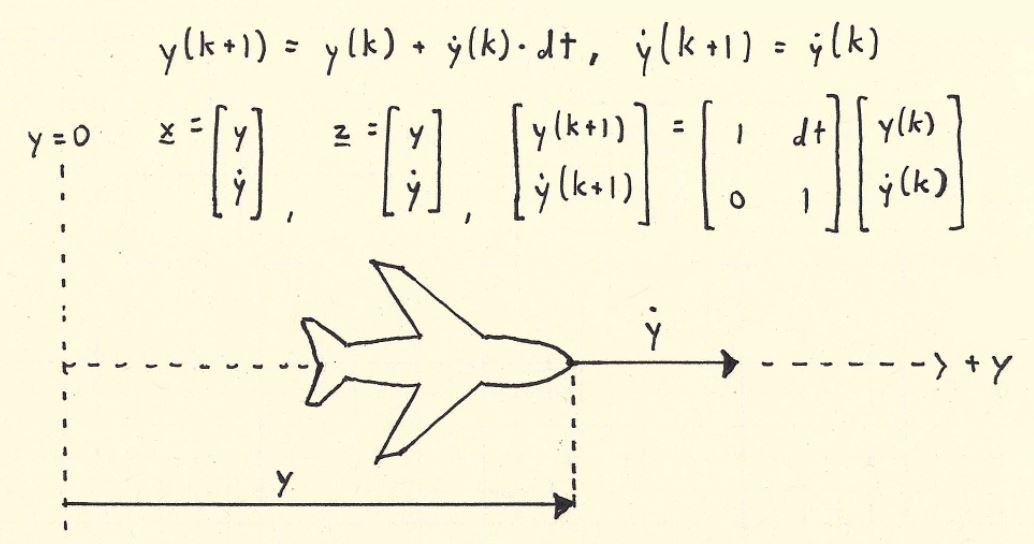
\includegraphics[width=\textwidth]{airplanediag}
	\caption{Airplane example diagram and equations of motion}
	\label{fig:airplanediag}
\end{figure}

The filter uses matrix operations and a state-space representation of the system model to allow for systems with various measurement and state dimensions. The state dimension \(n\) is the number of variables in the state vector, and the measurement dimension \(m\) is the number of variables in the state vector. The state vector \(\mathbf{x}_{n \times 1}\) is the collection of variables that the system is estimating. For the airplane example, the variables being estimated are the position \(y\) and the velocity \(\dot{y}\). The measurement vector \(\mathbf{z}_{m \times 1}\) is the collection of variables that are being measured \cite{kfsimply}. For the airplane example, the variables being measured are the position \(y\) (by the GPS) and the velocity \(\dot{y}\) (by the pitot tube). In this example, the measurement vector is the same as the state vector; this is not always the case! If only the GPS was used for measurements (no pitot tube for velocity), then the measurement vector would only contain \(y\).

The state transition matrix \(\mathbf{F}_{n \times n}\) describes how the current state of the system affects the next state of the system. In a discrete system (like those implemented on real-time embedded systems), the next state of the system is described by \(\mathbf{x}(k+1)\), where \(k\) represents the current iteration of the system; \(k=0\) is the initial iteration, \(k=1\) is the next step, and so on. The state transition matrix describes how the next state \(\mathbf{x}(k+1)\) is related to the current state \(\mathbf{x}(k)\), and it must satisfy Equation \ref{eq:stm}. Usually, this matrix is determined using the dynamics of the system \cite{kfsimply}. For the airplane example, the state transition matrix is shown in Figure \ref{fig:airplanediag}; it is derived from the equation of motion of the system, assuming particle motion (no drag) and constant velocity.

\begin{equation} \label{eq:stm}
	\mathbf{x}(k+1) = \mathbf{F} \mathbf{x}(k)
\end{equation}

The state-to-measurement matrix \(\mathbf{H}_{m \times n}\) describes how the current state of the system can be transformed to give the measurement of the system. This may seem counterintuitive; aren’t the measurements used to estimate the state of the system, and not the other way around? This is true, but the Kalman filter converts the current state estimate to equivalent measurements in the update step (and uses the difference between the estimated measurements and the true measurements to update its uncertainty) \cite{kfsimply}. This matrix must satisfy Equation \ref{eq:stmm}. For the airplane example, this matrix is quite simple; it is just a 2x2 identity matrix, since the measurement vector and state vector are the same in this case.

\begin{equation} \label{eq:stmm}
	\mathbf{z}(k) = \mathbf{H} \mathbf{x}(k)
\end{equation}

The state covariance matrix \(\mathbf{P}_{n \times n}\) is a dynamic estimate of the uncertainty in the state estimate of the system. Essentially, this matrix describes how confident the filter is in its estimate of the current state. This matrix is constantly updated as the filter is run and performs best if an initial uncertainty estimate is given \cite{kfsimply}. A good way to initialize this matrix is to populate it with the initial value of the process noise matrix (seen below). Initializing it with all zeros works too, but may lead to slower filter convergence.

The process noise matrix \(\mathbf{Q}_{n \times n}\) describes the assumed uncertainty of the state estimate of the system. This matrix describes how the actual system is affected by disturbances. Diagonal elements of the matrix represent the uncertainty/variance of each individual state variable, while the off-diagonal elements represent the covariance between state variables \cite{kfsimply}. Generally, the off-diagonal elements are set to zero unless the system dynamics are well understood. For the airplane example, wind may push the aircraft around in the air, or the airplane may accelerate using its engines; with the constant velocity model, a high uncertainty for velocity should be assumed to account for the acceleration of the aircraft. 

The measurement covariance matrix \(\mathbf{R}_{m \times m}\) describes the assumed uncertainty of the measurements. It describes how noisy the measurement values are. Similarly to the process noise matrix, the diagonal elements represent the uncertainty/variance of each individual measurement variable, while the off-diagonal elements represent the covariance between measurement variables. The Kalman filter model does assume normally-distributed noise across both measurements and state variables, so non-normal noise can cause the filter to be less accurate. If individual measurement devices have a known variance, these values can be used along the diagonal elements of the measurement covariance matrix \cite{kfsimply}. It is typically more difficult to measure the covariance between measurement devices, so the off-diagonal elements are usually set to zero. For the airplane example, the first and second diagonal elements of the measurement covariance matrix should be set to the variance of the GPS measurements and the pitot tube readings, respectively.

The final matrix used in the Kalman filter is the Kalman gain \(\mathbf{K}_{n \times m}\), which is used internally during the update step. It will be explained in more detail during the update step explanation.

The first step in running the Kalman filter (blocks 1 and 2 in Figure \ref{fig:kalmanbd}) is to initialize the state vector and the state covariance matrix. The state vector can be initialized using measurements (setting the initial position to the first GPS measurement and the initial velocity to the first pitot tube reading), or it can be set to zero (or some other constant value) \cite{kfsimply}. The first approach is recommended as it leads to faster convergence of the filter. However, the second approach was taken in the software implementation for simplicity. The state covariance matrix initialization is covered in its paragraph above.

\pagebreak

The next step (block 3) is to predict the next state of the system. This step can be run as often as desired; if a state estimate every 100ms is desired but measurements only arrive every two seconds, the prediction step can be run every 100ms and the update step can be run when a new measurement arrives. In this step, two equations are used: the first (Equation \ref{eq:p1}) predicts the next state of the system using the current state vector and the state transition matrix; the second (Equation \ref{eq:p2}) updates the state covariance matrix \cite{kfsimply}. The state covariance matrix grows in each prediction step, which should make sense; the more times the state is predicted without implementing measurements, the more uncertain the new state estimate is.

\begin{equation} \label{eq:p1}
	\mathbf{x}(k+1) = \mathbf{F} \mathbf{x}(k)
\end{equation}

\begin{equation} \label{eq:p2}
	\mathbf{P}(k+1) = \mathbf{F} \mathbf{P}(k) \mathbf{F}^T + \mathbf{Q}
\end{equation}

The last step (blocks 4 and 5) is to update the state estimate using new measurements. First, the estimated measurements are calculated; these are found by converting the current state estimate to equivalent measurements using the state-to-measurement matrix. The estimated measurement vector is subtracted from the (true) measurement vector in Equation \ref{eq:u1} to give the difference between the estimated and true measurements \cite{kfsimply}. This difference is represented by the vector \(\mathbf{y}\).

\begin{equation} \label{eq:u1}
	\mathbf{y} = \mathbf{z}(k) - \mathbf{H} \mathbf{x}(k)
\end{equation}

Next, the Kalman gain is computed. The Kalman gain is derived in Kálmán’s original paper \cite{kalman} and represents the optimal way to combine the current state estimate of the system, the new measurements, and the known uncertainties and dynamics of the system; it is calculated using Equation \ref{eq:u2}. The Kalman gain converts the difference between the estimated and true measurements \(\mathbf{y}\) to a change in the state estimate, which is then added to the current state estimate as shown in Equation \ref{eq:u3}. This sum is the next estimate of the state of the system \cite{kfsimply}.

\begin{equation} \label{eq:u2}
	\mathbf{K} = \mathbf{P}(k) \mathbf{H}^T (\mathbf{H} \mathbf{P}(k) \mathbf{H}^T + \mathbf{R})^{-1} 
\end{equation}

\begin{equation} \label{eq:u3}
	\mathbf{x}(k+1) = \mathbf{x}(k) + \mathbf{K} \mathbf{y}
\end{equation}

Finally, the state covariance matrix is updated using the Kalman gain as shown in Equation \ref{eq:u4} \cite{kfsimply}. Note that this step makes the state covariance matrix smaller; this should be expected, as measuring the system reduces the uncertainty in the state estimate.

\begin{equation} \label{eq:u4}
	\mathbf{P}(k+1) = \mathbf{P}(k) - \mathbf{K} \mathbf{H} \mathbf{P}(k)
\end{equation}

After initialization, the prediction and update steps can be run independently. For this particular implementation, both steps are run together; when a new acoustic position estimate becomes available, the prediction and update steps are run sequentially. This means that the Kalman filter only filters the noise between given position estimates - it doesn’t attempt to interpolate between measurements. If more frequent position estimates are desired (which they almost certainly would be for an underwater vehicle), then the prediction step can be run whenever new measurements are unavailable.

\section{Software Implementation} \label{sec:5s2}
The software implementation follows the theory in the previous section very closely. This section will describe the implementation on the STM32 for a general Kalman filter; the specifics of the initialization and dynamics for the two filters (only acoustic position estimates, and combined acoustic + dead reckoning estimates) are detailed in Sections \ref{sec:5s3} and \ref{sec:5s4}, respectively.

The matrix operations from the \verb|arm_math.h| library are used in this implementation due to the vast number of matrix operations required for the Kalman filter. This library was also used in Section \ref{ssec:3s8s2}, and is written for ARM Cortex cores \cite{arm}.

A custom struct is made for each Kalman filter; it contains pointers for every vector and matrix used in the Kalman filter.

\begin{lstlisting}[language=C++]
typedef struct {
	arm_matrix_instance_f32 x; // State estimate
	arm_matrix_instance_f32 P; // Estimate covariance
	arm_matrix_instance_f32 F; // State transition matrix
	arm_matrix_instance_f32 H; // Measurement matrix
	arm_matrix_instance_f32 Q; // Process noise covariance
	arm_matrix_instance_f32 R; // Measurement noise covariance
	arm_matrix_instance_f32 K; // Kalman gain
	
	float32_t *x_data;
	float32_t *P_data;
	float32_t *F_data;
	float32_t *H_data;
	float32_t *Q_data;
	float32_t *R_data;
	float32_t *K_data;
	
	size_t state_dim;
	size_t meas_dim;
} KalmanFilter;
\end{lstlisting}

Initializing a \verb|KalmanFilter| struct is fairly involved, so a custom function was written to simplify the process. The function takes in pointers to various \verb|float32_t| lists and writes the values of those lists to the various vectors and matrices in the \verb|KalmanFilter| struct. Refer to Sections \ref{sec:5s3} and \ref{sec:5s4} to see how a \verb|KalmanFilter| struct is initialized with given \verb|float32_t| lists.

\pagebreak

\begin{lstlisting}[language=C++]
void kalman_filter_init(KalmanFilter* kf, float32_t* x_values, float32_t* P_values, float32_t* F_values, float32_t* H_values, float32_t* Q_values, float32_t* R_values) {
	memcpy(kf->x_data, x_values, kf->state_dim * sizeof(float32_t));
	memcpy(kf->P_data, P_values, kf->state_dim * kf->state_dim * sizeof(float32_t));
	memcpy(kf->F_data, F_values, kf->state_dim * kf->state_dim * sizeof(float32_t));
	memcpy(kf->H_data, H_values, kf->meas_dim * kf->state_dim * sizeof(float32_t));
	memcpy(kf->Q_data, Q_values, kf->state_dim * kf->state_dim * sizeof(float32_t));
	memcpy(kf->R_data, R_values, kf->meas_dim * kf->meas_dim * sizeof(float32_t));
}
\end{lstlisting}

The prediction step is handled with the function \verb|kalman_filter_predict()|, which takes the pointer to the \verb|KalmanFilter| struct as an input. This step implements Equations \ref{eq:p1} and \ref{eq:p2} from Section \ref{ssec:5s1s2}. Temporary matrices are used to hold some of the outputs; it is imperative that these matrix instances are freed from memory after the prediction step is run, or else a memory leak will occur.

\begin{lstlisting}[language=C++]
void kalman_filter_predict(KalmanFilter* kf) {
	// Temporary matrices
	float32_t* temp_state = (float32_t*)malloc(kf->state_dim * sizeof(float32_t));
	float32_t* temp_cov = (float32_t*)malloc(kf->state_dim * kf->state_dim * sizeof(float32_t));
	float32_t* temp_F_transpose = (float32_t*)malloc(kf->state_dim * kf->state_dim * sizeof(float32_t));
	
	arm_matrix_instance_f32 temp_state_mat, temp_cov_mat, F_transpose_mat;
	
	arm_mat_init_f32(&temp_state_mat, kf->state_dim, 1, temp_state);
	arm_mat_init_f32(&temp_cov_mat, kf->state_dim, kf->state_dim, temp_cov);
	arm_mat_init_f32(&F_transpose_mat, kf->state_dim, kf->state_dim, temp_F_transpose);
	
	// x = F * x
	arm_mat_mult_f32(&kf->F, &kf->x, &temp_state_mat);
	memcpy(kf->x_data, temp_state, kf->state_dim * sizeof(float32_t));
	
	// P = F * P * F^T + Q
	arm_mat_mult_f32(&kf->F, &kf->P, &temp_cov_mat);
	arm_mat_trans_f32(&kf->F, &F_transpose_mat);
	arm_mat_mult_f32(&temp_cov_mat, &F_transpose_mat, &kf->P);
	arm_mat_add_f32(&kf->P, &kf->Q, &kf->P);
	
	free(temp_state);
	free(temp_cov);
	free(temp_F_transpose);
}
\end{lstlisting}

The update step is handled with the function \verb|kalman_filter_update()|, which takes the pointer to the \verb|KalmanFilter| struct and the pointer to a \verb|float32_t| list of measurements as inputs. This step implements Equations \ref{eq:u1} through \ref{eq:u4} from Section \ref{ssec:5s1s2}; some of these equations have been simplified or split into multiple chunks for ease of implementation. Many temporary matrices are used for intermediate calculations and their instances must be freed from memory after running the update function, or else memory leaks will occur.

\begin{lstlisting}[language=C++]
void kalman_filter_update(KalmanFilter* kf, float32_t* measurement) {
	// Temporary matrices
	float32_t* temp_state = (float32_t*)malloc(kf->state_dim * sizeof(float32_t));
	float32_t* temp_measure = (float32_t*)malloc(kf->meas_dim * sizeof(float32_t));
	float32_t* temp_H_P = (float32_t*)malloc(kf->meas_dim * kf->state_dim * sizeof(float32_t));
	float32_t* temp_H_transpose = (float32_t*)malloc(kf->state_dim * kf->meas_dim * sizeof(float32_t));
	float32_t* temp_P_H_transpose = (float32_t*)malloc(kf->state_dim * kf->meas_dim * sizeof(float32_t));
	float32_t* temp_S = (float32_t*)malloc(kf->meas_dim * kf->meas_dim * sizeof(float32_t));
	float32_t* temp_S_inv = (float32_t*)malloc(kf->meas_dim * kf->meas_dim * sizeof(float32_t));
	float32_t* temp_K_H = (float32_t*)malloc(kf->state_dim * kf->state_dim * sizeof(float32_t));
	float32_t* temp_K_H_P = (float32_t*)malloc(kf->state_dim * kf->state_dim * sizeof(float32_t));
	
	arm_matrix_instance_f32 temp_state_mat, temp_measure_mat, temp_H_P_mat, H_transpose_mat, P_H_transpose_mat, S_mat, S_inv_mat, K_H_mat, K_H_P_mat;
	
	arm_mat_init_f32(&temp_state_mat, kf->state_dim, 1, temp_state);
	arm_mat_init_f32(&temp_measure_mat, kf->meas_dim, 1, temp_measure);
	arm_mat_init_f32(&temp_H_P_mat, kf->meas_dim, kf->state_dim, temp_H_P);
	arm_mat_init_f32(&H_transpose_mat, kf->state_dim, kf->meas_dim, temp_H_transpose);
	arm_mat_init_f32(&P_H_transpose_mat, kf->state_dim, kf->meas_dim, temp_P_H_transpose);
	arm_mat_init_f32(&S_mat, kf->meas_dim, kf->meas_dim, temp_S);
	arm_mat_init_f32(&S_inv_mat, kf->meas_dim, kf->meas_dim, temp_S_inv);
	arm_mat_init_f32(&K_H_mat, kf->state_dim, kf->state_dim, temp_K_H);
	arm_mat_init_f32(&K_H_P_mat, kf->state_dim, kf->state_dim, temp_K_H_P);
	
	// y = z - H * x
	arm_mat_mult_f32(&kf->H, &kf->x, &temp_measure_mat);
	arm_sub_f32(measurement, temp_measure, temp_measure, kf->meas_dim);
	
	// S = H * P * H^T + R
	arm_mat_mult_f32(&kf->H, &kf->P, &temp_H_P_mat);
	arm_mat_trans_f32(&kf->H, &H_transpose_mat);
	arm_mat_mult_f32(&temp_H_P_mat, &H_transpose_mat, &S_mat);
	arm_mat_add_f32(&S_mat, &kf->R, &S_mat);
	
	// K = P * H^T * S^-1
	arm_mat_inverse_f32(&S_mat, &S_inv_mat);
	arm_mat_mult_f32(&kf->P, &H_transpose_mat, &P_H_transpose_mat);
	arm_mat_mult_f32(&P_H_transpose_mat, &S_inv_mat, &kf->K);
	
	// x = x + K * y
	arm_mat_mult_f32(&kf->K, &temp_measure_mat, &temp_state_mat);
	arm_add_f32(kf->x_data, temp_state, kf->x_data, kf->state_dim);
	
	// P = (I - K * H) * P
	arm_mat_mult_f32(&kf->K, &kf->H, &K_H_mat);
	arm_mat_mult_f32(&K_H_mat, &kf->P, &K_H_P_mat);
	arm_mat_sub_f32(&kf->P, &K_H_P_mat, &kf->P);
	
	free(temp_state);
	free(temp_measure);
	free(temp_H_P);
	free(temp_H_transpose);
	free(temp_P_H_transpose);
	free(temp_S);
	free(temp_S_inv);
	free(temp_K_H);
	free(temp_K_H_P);
}
\end{lstlisting}

Finally, one function was created to update the state transition and state-to-measurement matrices for both Kalman filters used in this thesis. As in the airplane example in Section \ref{ssec:5s1s2}, the system dynamics of the iSBL array are dependent on the change in time between updates, \verb|dt|. This variable is found in the state transition matrix for both Kalman filter systems, and is found in the state-to-measurement matrix of the iSBL-SF filter.

\begin{lstlisting}[language=C++]
void update_kalman_matrices(KalmanFilter* kf_combined, KalmanFilter* kf_isbl, float32_t dt) {
	// Update F matrix for all KalmanFilters
	// Assuming F is a 6x6 matrix for all filters
	kf_combined->F_data[3] = dt;
	kf_combined->F_data[10] = dt;
	kf_combined->F_data[17] = dt;
	
	kf_isbl->F_data[3] = dt;
	kf_isbl->F_data[10] = dt;
	kf_isbl->F_data[17] = dt;
	
	// Update H matrix for combined KF (6x6)
	kf_combined->H_data[21] = dt;
	kf_combined->H_data[28] = dt;
	kf_combined->H_data[35] = dt;
	
	// No update needed for iSBL KF H matrix
}
\end{lstlisting}

The above functions are used in the main loop of the STM32 receiver code, during the data processing state (see Section \ref{ssec:3s7s1} for the finite-state machine representation of the system). Both Kalman filters are initialized in the initialization state of the program.

After the acoustic position estimate is returned (as mentioned at the end of Section \ref{ssec:3s9s3}), the change in time since the last acoustic position estimate is calculated using timer TIM14. This timer has a prescalar of 65536 and a period of 65536; it ticks at approximately 4.12kHz and has an overall period of approximately 15.62s. An acoustic pulse is sent from the transmitter to the receiver once per second, and without any artificial delays the STM32 is able to convert the recordings to a position estimate in under one second; for testing, delays were added to prevent recordings when the Fo-SHIP was moving between different positions. This means that the STM32 is able to miss up to 14 acoustic pulses before the timer overflows. In testing, this never occurred, but should be reconsidered for a full underwater implementation. Adding a simple counter (that increments each time the period is exceeded) would be an easy way to fix this issue.

\begin{lstlisting}[language=C++]
else if (state == 4){
	...
	// subtract estimated position to transmitter from known transmitter location to get receiver position in global frame
	raw_isbl_pos_est.x = true_x - raw_isbl_pos_est.x;
	raw_isbl_pos_est.y = true_y - raw_isbl_pos_est.y;
	raw_isbl_pos_est.z = true_z - raw_isbl_pos_est.z;
	
	// calculate the change in time since the last acoustic update (deltat_pos)
	timestamp2 = __HAL_TIM_GET_COUNTER(&htim14);
	uint32_t diff_ticks;
	if (timestamp2 >= previousTimestamp2) {
		diff_ticks = timestamp2 - previousTimestamp2;
	} else {
		diff_ticks = (65536 - previousTimestamp2) + timestamp2;
	}
	deltat_pos = (float)diff_ticks * 65536.0f / 275000000.0f;
	previousTimestamp2 = __HAL_TIM_GET_COUNTER(&htim14);
\end{lstlisting}

Next, the relevant state transition and state-to-measurement matrices are updated with the new change in time.

\begin{lstlisting}[language=C++]
	update_kalman_matrices(kf_combined, kf_isbl, deltat_pos);
\end{lstlisting}

After this, the prediction steps for both filters are run.

\begin{lstlisting}[language=C++]
	kalman_filter_predict(kf_combined);
	kalman_filter_predict(kf_isbl);
\end{lstlisting}

Then, the measurement vectors for each filter are populated, and the update step is run for both filters.

\begin{lstlisting}[language=C++]
	// get measurements
	float32_t measurements_combined[6] = {
		raw_isbl_pos_est.x, raw_isbl_pos_est.y, raw_isbl_pos_est.z, delta_x_imu.x, delta_x_imu.y, delta_x_imu.z
	};
	float32_t measurements_isbl[3] = {
		raw_isbl_pos_est.x, raw_isbl_pos_est.y, raw_isbl_pos_est.z
	};
	
	// update step for filters
	kalman_filter_update(kf_combined, measurements_combined);
	kalman_filter_update(kf_isbl, measurements_isbl);
\end{lstlisting}

At this point, the state estimates are stored in the \verb|x_data[]| vectors inside of each \verb|KalmanFilter| struct. These estimates are converted from units of meters to millimeters (to match the Fo-SHIP position units and to reduce the number of characters sent between the STM32 and ESP32). 

\begin{lstlisting}[language=C++]
	kf_comb_pos_est.x = kf_combined->x_data[0] * 1000;
	kf_comb_pos_est.y = kf_combined->x_data[1] * 1000;
	kf_comb_pos_est.z = kf_combined->x_data[2] * 1000;
	
	kf_isbl_pos_est.x = kf_isbl->x_data[0] * 1000;
	kf_isbl_pos_est.y = kf_isbl->x_data[1] * 1000;
	kf_isbl_pos_est.z = kf_isbl->x_data[2] * 1000;
\end{lstlisting}

The other position estimates (the raw acoustic position estimate and the true position of the transmitter) are also converted to millimeters in this step.

Finally, all of the position estimates are sent over the serial connection to the ESP32 for data logging. The details of each position estimate are covered in Chapter \ref{chap:6c}, where the data collection and test plan is discussed.

After this step, the STM32 re-enters the triggering state and restarts the whole process (from Chapter \ref{chap:3c} to this chapter) over again!

\section{iSBL Kalman Filter Design} \label{sec:5s3}
Two Kalman filters are being tested for this thesis: one that just filters the acoustic position estimates, and one that combines the acoustic position estimates with the change-in-position estimates of the dead reckoning system. The first filter will be referred to as the “iSBL filter,” and the second will be referred to as the “iSBL-SF filter” (Inverted Short Baseline - Sensor Fusion, to note that multiple sensor estimates are being fused together). This section will detail the first filter, but both filters are quite similar; it is advised to read this section before Section \ref{sec:5s3}.

The system dynamics of the iSBL filter are very similar to the airplane example in Section \ref{ssec:5s1s2}, just extrapolated to three dimensions. The system is assumed to have constant velocity, particle motion (tracking the center of the iSBL array), and independent motion along each of its three axes (X, Y, and Z); Section \ref{ssec:5s1s2} covers these assumptions in more detail. It is also assumed that the particle moves in the test frame defined in Section \ref{ssec:3s9s1}. In total, six equations define the dynamics of the iSBL array:

\begin{equation} \label{eq:isbl1}
	x(k+1) = x(k) + \Delta t \dot{x}(k)
\end{equation}

\begin{equation} \label{eq:isbl2}
	\dot{x}(k+1) = \dot{x}(k)
\end{equation}

\begin{equation} \label{eq:isbl3}
	y(k+1) = y(k) + \Delta t \dot{y}(k)
\end{equation}

\begin{equation} \label{eq:isbl4}
	\dot{y}(k+1) = \dot{y}(k)
\end{equation}

\begin{equation} \label{eq:isbl5}
	z(k+1) = z(k) + \Delta t \dot{z}(k)
\end{equation}

\begin{equation} \label{eq:isbl6}
	\dot{z}(k+1) = \dot{z}(k)
\end{equation}

The position of the iSBL array’s center along the x-axis at timestep \(k\) is given by \(x(k)\) and its velocity along the x-axis is given by \(\dot{x}(k)\); the same holds for the y- and z-axes. The state vector, \(\mathbf{x}\), is defined below in Equation \ref{eq:isbl7}. 

\begin{equation} \label{eq:isbl7}
	\mathbf{x} = [x, y, z, \dot{x}, \dot{y}, \dot{z}]^T
\end{equation}

Thus, the state vector and state transition matrix for the iSBL array are given as the following:

\begin{lstlisting}[language=C++]
float32_t x_values[6] = {0, 0, 0, 0, 0, 0};

float32_t F_values[6 * 6] = {
	1, 0, 0, 1, 0, 0,
	0, 1, 0, 0, 1, 0,
	0, 0, 1, 0, 0, 1,
	0, 0, 0, 1, 0, 0,
	0, 0, 0, 0, 1, 0,
	0, 0, 0, 0, 0, 1
};
\end{lstlisting}

Note that the state vector \(x\) is a column vector and only appears as a row vector here; these are lists that will be used to initialize the \verb|KalmanFilter| struct, as described in Section \ref{sec:5s2}. Also note that the change in time, \(\Delta t\), is currently replaced with 1s. Section \ref{sec:5s2} notes how the change in time can differ with each filter update and how the function \verb|update_kalman_matrices()| addresses this.

Next, the state covariance matrix is initialized with 10s along the diagonal. This is fairly arbitrary; it represents a moderate uncertainty of the initial state estimate (which is all zeros). It could easily be replaced with the process noise matrix, but the initial uncertainty in position is reflected better in this manner.

\begin{lstlisting}[language=C++]
float32_t P_values[6 * 6] = {
	10, 0, 0, 0, 0, 0,
	0, 10, 0, 0, 0, 0,
	0, 0, 10, 0, 0, 0,
	0, 0, 0, 10, 0, 0,
	0, 0, 0, 0, 10, 0,
	0, 0, 0, 0, 0, 10
};
\end{lstlisting}

The process noise matrix is set to describe the uncertainty in the system dynamics. As the position along each axis is fairly well described by the model, the corresponding values in the matrix are relatively small. However, the equations for velocity are not very accurate; they assume that the velocity never changes. This is, of course, not the case with the Fo-SHIP moving the iSBL array around. The process noise for the velocity variables is set higher to account for this.

\begin{lstlisting}[language=C++]
float32_t Q_values[6 * 6] = {
	.1, 0, 0, 0, 0, 0,
	0, .1, 0, 0, 0, 0,
	0, 0, .1, 0, 0, 0,
	0, 0, 0, 10, 0, 0,
	0, 0, 0, 0, 10, 0,
	0, 0, 0, 0, 0, 10
};
\end{lstlisting}

The above matrices and variables are the same for both the iSBL filter and the iSBL-SF filter; the system dynamics aren’t changing, only the measurements are. The following three matrices and vectors differ between the two filters.

First, the measurement vector for the iSBL filter is only populated with acoustic position estimates. The acoustic positioning system returns a 3D position estimate for the center of the array, and the state-to-measurement matrix reflects that. The measurement vector, \(\mathbf{z}\), is defined below in Equation \ref{eq:isbl8}, and the definition of the state-to-measurement matrix is shown in the code block below.

\begin{equation} \label{eq:isbl8}
	\mathbf{z} = [x, y, z]^T
\end{equation}

\begin{lstlisting}[language=C++]
float32_t H_values[3 * 6] = {
	1, 0, 0, 0, 0, 0,
	0, 1, 0, 0, 0, 0,
	0, 0, 1, 0, 0, 0
};
\end{lstlisting}

Finally, the measurement noise matrix represents the uncertainty in each of the measurements. In a full underwater implementation, these values should be replaced with the true variance of the position estimate, and the other matrices should be scaled around them. For this implementation, a value of 1000 along the diagonal was found to give decent results. Section \ref{sec:5s5} discusses this tuning further.

\begin{lstlisting}[language=C++]
float32_t R_values[3 * 3] = {
	1000, 0, 0,
	0, 1000, 0,
	0, 0, 1000
};
\end{lstlisting}

All of the above matrices reside inside of \verb|init_kalman_filter_isbl()|, the initialization function for this filter. This function is called during the initialization state of the program and sets up the \verb|KalmanFilter| struct associated with this filter.

\begin{lstlisting}[language=C++]
KalmanFilter* init_kalman_filter_isbl() {
	float32_t x_values[6] = {0, 0, 0, 0, 0, 0};
	...
	KalmanFilter* kf = create_kalman_filter(6, 3);
	kalman_filter_init(kf, x_values, P_values, F_values, H_values, Q_values, R_values);
	return kf;
}
\end{lstlisting}

\section{iSBL-SF Kalman Filter Design} \label{sec:5s4}
The iSBL-SF filter is truly the culmination of all the work done for this thesis: it combines the acoustic position estimate with the dead reckoning change-in-position estimate, both of which use the orientation estimate provided by the Madgwick filter. This filter is quite similar to the normal iSBL filter: it shares the same state vector, state transition matrix, state covariance matrix, and process noise matrix, since both filters are designed for the same physical system. The difference is in the measurement; here, the measurement vector is defined as shown in Equation \ref{eq:isblsf1}.

\begin{equation} \label{eq:isblsf1}
	\mathbf{z} = [x, y, z, \Delta x, \Delta y, \Delta z]^T
\end{equation}

Note that this is very similar to the state vector in Equation \ref{eq:isbl7}; the only difference is that the velocity terms are swapped for change-in-position terms. However, particle kinematics provides a convenient solution to this: the change in position of a particle is equal to its velocity times the change in time, as seen in Equation \ref{eq:isblsf2}. 

\begin{equation} \label{eq:isblsf2}
	\Delta x = \Delta t \times \dot{x}
\end{equation}

The state-to-measurement matrix transforms the state variables into measurement variables. So, the first three diagonal elements should be set to one (the first three variables of both the state and measurement vector are the same), while the last three diagonal elements should be set to the change in time since the last filter update, \(\Delta t\). Note that in the initialization, these last three diagonal elements are set to one; they are updated with the proper \(\Delta t\) during the update step, as described in Section \ref{sec:5s2}.

\begin{lstlisting}[language=C++]
float32_t H_values[6 * 6] = {
	1, 0, 0, 0, 0, 0,
	0, 1, 0, 0, 0, 0,
	0, 0, 1, 0, 0, 0,
	0, 0, 0, 1, 0, 0,
	0, 0, 0, 0, 1, 0,
	0, 0, 0, 0, 0, 1
};
\end{lstlisting}

Finally, the measurement noise matrix should represent the uncertainty in each of the measurements. For simplicity, the first three diagonal elements (uncertainty in acoustic position estimates) are the same as the iSBL filter. The dead reckoning system is much less accurate (as shown in Section \ref{sec:4s6}), and this is reflected with a much higher value in the last three diagonal elements. The dead reckoning estimate is likely more than 10x less accurate than the position estimate, but anything larger than this resulted in no meaningful difference between the iSBL filter and the iSBL-SF filter. Even with this measurement noise matrix, both filters are very similar; a better dead reckoning change-in-position estimate (using doppler velocity logs, better orientation estimates and accelerometers, etc.) is highly recommended for a full underwater implementation.

\begin{lstlisting}[language=C++]
float32_t R_values[6 * 6] = {
	1000, 0, 0, 0, 0, 0,
	0, 1000, 0, 0, 0, 0,
	0, 0, 1000, 0, 0, 0,
	0, 0, 0, 10000, 0, 0,
	0, 0, 0, 0, 10000, 0,
	0, 0, 0, 0, 0, 10000
};
\end{lstlisting}

These matrices (and the state matrices described in Section \ref{sec:5s3}) are housed in \verb|init_kalman_filter_combined()|, the initialization function for this filter. Similarly to the iSBL filter, this function is called during the initialization state of the program.

\begin{lstlisting}[language=C++]
KalmanFilter* init_kalman_filter_combined(void) {
	float32_t x_values[6] = {0, 0, 0, 0, 0, 0};
	..
	KalmanFilter* kf = create_kalman_filter(6, 6);
	kalman_filter_init(kf, x_values, P_values, F_values, H_values, Q_values, R_values);
	return kf;
}
\end{lstlisting}

\section{Filter Tuning} \label{sec:5s5}
Tuning a Kalman filter is a very important step towards getting good results; unfortunately, it is much more difficult than tuning a Madgwick filter (see Section \ref{sec:4s6} for that tuning process). For each Kalman filter, there are three matrices that require tuning:
\begin{itemize}[noitemsep,topsep=0pt,]
	\item The state covariance matrix
	\item The measurement noise matrix
	\item The process noise matrix
\end{itemize}

The state covariance matrix generally requires the least tuning of the three; a good initial estimate is recommended (copying the process noise matrix is usually a good first step), but it updates as the filter iterates and tends to converge as the state estimate does. Tuning the state covariance matrix results in faster convergence of the filter, and helps to prevent divergence.

\pagebreak

The measurement noise matrix is most straightforward of the three to tune. If all of the measurement devices can be tested before the filter is implemented, it is possible to construct this matrix with the variance and covariance of each measurement sensor. Note that the Kalman filter assumes a normal distribution for each of the variances; this can be problematic if the noise is not normally-distributed. Section \ref{sec:6s3} touches upon this and explores the normality of the acoustic position measurements. 

To find the variance of a particular sensor, it is recommended to take as many static measurements as possible, and to vary them through the range of the sensor. For example, to find the measurement noise of a pressure sensor used for estimating the depth of a submarine, it may be useful to hold the sensor at different depth intervals for a set period of time. The measurements for one depth interval can be analyzed and the variance of the measurements can be estimated; for best results, it may even be possible to fit the variance to a function that changes with the state of the system (perhaps the sensor is noisier at greater depths). Otherwise, the sensor measurements can be averaged across the range of the sensor, and a single constant variance can be determined.

This process was not performed for the iSBL filter or the iSBL-SF filter; time simply ran out. The measurement noise matrix values were refined through testing and are presented as a “good enough” solution. For a full underwater implementation, properly tuning the Kalman filter is highly encouraged.

Finally, the process noise matrix is the most difficult of the three to tune. It represents the uncertainty in the system model, something that is hard to quantify. It is recommended to tune this matrix after tuning the others. In general, the tunable matrices of a Kalman filter are relative to each other; each value in each matrix has proper units and technically has a real-world meaning, but the process noise is often difficult to relate to real-world measurements. Also, the assumptions made for the system dynamics can be used to inform the process noise matrix tuning. For example, in a constant velocity model, the uncertainty for the velocity state will likely be larger if the system is frequently accelerating.

Methods for automating the tuning of Kalman filters do exist, and many use experimental and quantitative data to do so \cite{kftuning}. However, these tuning methods often only work for linear Kalman filters, so applications may be limited. These guidelines were developed during the tuning process for this thesis:
\begin{itemize}[noitemsep,topsep=0pt,]
	\item Start with the measurement noise matrix, use the relative variance of the measurements as an initial guess
	\item Modify the process noise matrix, taking into account the assumptions made about the system dynamics
	\item Set the state covariance matrix to the process noise matrix, and modify based on the initial condition of the system relative to its first “converged” state estimate
	\item Check for divergence of the Kalman filter (usually when process uncertainties are too high)
	\item Repeat the tuning for each matrix, noting the convergence speed, stability of the state estimate, and accuracy of the state estimate (if applicable)
\end{itemize}

\bibliographystyle{IEEEtran}
\bibliography{../thesis}

\end{document}